\documentclass{article}
\usepackage{graphicx}
\begin{document}
\section{Summary}
The game is a simple top-down shooter where the players are in control of humans
that must fight off an endless horde of zombies.  The world is a single quad
surrounded on all sides by insurmountable walls.  Zombies spawn in waves
randomly around the area, getting faster and more numerous as time goes on.  To
kill the zombies each player is equipped with a gun that they may fire every
second --- most zombies die in just one hit, but larger ones take multiple hits.

\begin{figure}[h!]
\centering
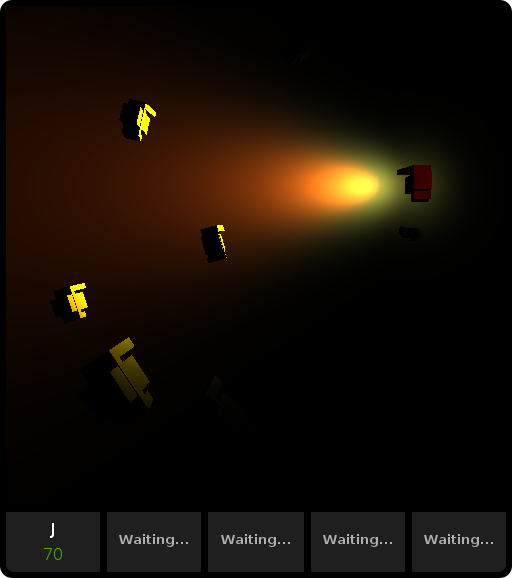
\includegraphics[width=0.75\linewidth]{zombies.png}
\caption{The player fires a shot into a horde of zombies.}
\end{figure}

\section{Network Utilization}
The game is implemented in the browser and as such uses typical techniques found
in that domain.  The server is a very basic \textit{HTTP} server (\texttt{AJAXServer})
that translates certain requests into
method calls on the game server (\texttt{Server}) and the client is a web page
that uses \textit{AJAX} to communicate with the server without reloading the page.

The server-to-client packets are defined in \texttt{src/server/AJAXConnection.java}
lines 9--175.  They are implemented in a JSONP-inspired manner, the client requests
the page \texttt{/update} and the server turns all the packets waiting to be
sent to the client into a series of function calls to be executed by the
client's JavaScript engine (for example \texttt{PingSPacket} becomes the code
\texttt{handlePing();}).  This technique is known as long-polling and is a
common approach to circumventing the client-server architecture of the web; in
the future websockets would be a more appropriate medium for communicating
between the server and client.

The client-to-server packets are defined in \texttt{src/client/index} lines
149--159, 164--168.  They are implemented as simple HTTP POST requests with the
body of the request containing the data of the packet.  The server parses out
these requests and turns them into packets (177--206) which are placed on the
queue of the associated \texttt{AJAXConnection} object and translated into
method calls on \texttt{Server} such as \texttt{handleJoin}.

See the attached document describing the flow of data across the network.

\section{Client Implementation}
The client is implemented in \texttt{src/client/index} as an HTML5 page containing
inline JavaScript and CSS and is a thin wrapper around the data structures
provided by the server,
although it does some basic simulation itself so that network load can be
reduced.  The bulk of the code handles the rendering of the game state
(281--600), followed by the networking code (149--279) and the data structures
manipulated by these two modules (91--119).

\begin{tabular}{r|l}
\textbf{Data Type} & \textbf{Use} \\
\hline
Player & Contains the name, position and velocity of the players and enemies.\footnotemark[1] \\
Wall & Contains the position, width and height of the impassable walls. \\
Shot & Contains the position, velocity and network id of the shots fired by the players. \\
PlayerObject & Contains the model and lights used to render the player. \\
EnemyObject & Contains the model used to render the enemy. \\
ShotObject & Contains the light used to render the flash of a shot being fired.
\end{tabular}

\footnotetext[1]{Enemies have an additional network id property.  The player that is being controlled by the user has properties that control the inputs that will be passed to the server (i.e. movement direction).}

\subsection{Assets}
The assets used in this game were lifted from another module's work and are the
work of Martin Griffin (modeling) and Robert Griffin (audio).

\section{Server Implementation}
The game-related parts of the server is implemented chiefly in \texttt{src/server/Server.java}
and \texttt{src/server/Game.java}.  These objects make use of \texttt{AJAXConnection}
to communicate with the clients that are playing the game, and \texttt{AJAXServer}
to accept new clients.

\begin{tabular}{r|l}
\textbf{Data Type} & \textbf{Use} \\
\hline
Player & Contains the state of a player/enemy and has methods to simulate, \\
& accept inputs from the network and try to attack. \\
Shot & Contains the position and velocity of a shot and its liveness. \\
Wall & Contains the position, width and height of a wall. \\
\end{tabular}

\section{Critical Review}
Generally the code is of poor quality and in dire need of refactoring.  Classes
such as \texttt{Game} have far more responsibilities than is reasonable; in
addition to handling game rules it also implements collision detection, AI and
network communication.  Even within the functions that are appropriate for the
class to own there is often severe deficiencies in that the code is overly long
and often repetitive in a way that suggests that the behavior should be extracted
out into a method of its own; this is shown most clearly in \texttt{Game::update}
where there are a number of loops that check for and handle collisions rather than
a generic \texttt{collidesWith} method on the entities involved in the collisions.  Of course
such a method would be impossible to implement due to none of the entities inheriting
from a common base class, rendering them all essentially separate from a code
perspective.

While there is some use of libraries on the client-side, the server is in much
need of the use of third-party libraries to deal with HTTP connections among other
concerns; the haphazard approach used to implement HTTP currently means that
connections are always closed (a source of gigantic latency) and almost all
HTTP headers are ignored.  Additionally it is trivial to crash the server by
providing malformed input or lying in the \texttt{Content-Length} header of
POST requests.

The client implementation is of a better overall quality but suffers from some
notable warts.  Firstly the entire page is specified in one file, destroying the
client's ability to cache the file and severely reducing maintainability.  Secondly
certain operations are intertwined, the rendering loop not only renders the scene
but also simulates the physics and (if a bot is playing) updating the AI --- this
grouping of unrelated functionality prevents the use of \texttt{requestAnimationFrame},
the standard way of having a callback that updates the scene.

There is however a diamond in the rough in the connection abstraction; the ability
to pretend that there is always a connection open to the client simplifies the
logic in \texttt{Server} considerably.  Additionally the abstraction is a stone's
throw away from allowing non-HTTP clients, the public methods of \texttt{AJAXConnection}
need only be lifted up into an interface \texttt{Connection} and then a pair of
(for example) \texttt{UDPServer} and \texttt{UDPConnection} could be defined that
marshal UDP packets into method calls on the server.  The server could transparently
accept HTTP and other clients in the same game instance.
\end{document}
